\chapter{MATERIAIS E MÉTODOS}
Esta seção apresenta os materiais e métodos utilizados no desenvolvimento do
JurisFlow, uma plataforma web destinada ao gerenciamento de informações e atividades
de escritórios de advocacia. São apresentados o ambiente tecnológico utilizado, as etapas
adotadas durante o desenvolvimento, o levantamento e a organização dos requisitos, a
modelagem do banco de dados, a implementação do módulo inicial e os procedimentos
utilizados para a verificação do sistema. A definição dos materiais e métodos considerou as
funcionalidades estabelecidas na proposta do projeto, bem como o refinamento do escopo
realizado ao longo do desenvolvimento. O sistema foi planejado com o objetivo de centralizar informações relacionadas a usuários, clientes, pastas, processos, diligências, prazos,
notificações e histórico de atividades, buscando contribuir para uma maior organização e
controle das atividades do escritório. Dessa forma, os procedimentos adotados foram estruturados de modo a acompanhar as etapas de construção da plataforma, desde a definição
dos requisitos até a implementação e verificação das funcionalidades desenvolvidas.

\section{MATERIAIS E FERRAMENTAS UTILIZADAS}
O desenvolvimento do JurisFlow contou com ferramentas de programação, controle de versão, modelagem de dados, organização de tarefas e verificação das requisições da aplicação. A seleção dessas ferramentas considerou as necessidades do projeto e a possibilidade de organizar o código-fonte, estruturar os dados e acompanhar as atividades da equipe.

O Visual Studio Code foi utilizado como ambiente de desenvolvimento, oferecendo suporte à edição dos arquivos e à utilização de extensões. O Git foi empregado para o controle de versão, enquanto o GitHub foi utilizado para hospedar o repositório e compartilhar o código-fonte entre os integrantes. Para a organização das atividades, utilizou-se o Trello. A modelagem do banco de dados foi realizada no dbdiagram.io, e o PlantUML foi utilizado na elaboração dos diagramas de casos de uso. Para testar as rotas da API, utilizou-se a extensão Thunder Client, integrada ao Visual Studio Code.

O PostgreSQL foi adotado como sistema gerenciador de banco de dados. O Docker foi utilizado para executar o banco de dados em um ambiente conteinerizado, contribuindo para padronizar a configuração de desenvolvimento.


\section{TECNOLOGIAS DE DESENVOLVIMENTO}
O desenvolvimento do JurisFlow utilizou JavaScript como principal linguagem de programação para a implementação da lógica da aplicação. A escolha dessa linguagem está relacionada à sua utilização no desenvolvimento web e à possibilidade de empregá-la tanto no frontend quanto no backend. Essa característica permite utilizar a mesma linguagem em diferentes partes da aplicação. Conforme apontam Cruz et al. (2018), o JavaScript deixou de ser utilizado exclusivamente em aplicações executadas em navegadores e passou a ser empregado também no desenvolvimento de outros tipos de software, incluindo aplicações para dispositivos móveis e computadores.

Para a implementação do backend, foi utilizado o Node.js, ambiente de execução que permite executar código JavaScript fora do navegador. Sua arquitetura é orientada a eventos e utiliza operações de entrada e saída não bloqueantes, características que favorecem o processamento de múltiplas requisições. Segundo Godinho (2023), a utilização do Node.js no desenvolvimento de aplicações está relacionada, entre outros aspectos, ao desempenho proporcionado pelo motor V8, desenvolvido pelo Google. No JurisFlow, o Node.js foi empregado no processamento das requisições e na comunicação entre a aplicação e o banco de dados.

O Visual Studio Code foi utilizado como ambiente de desenvolvimento por oferecer recursos de edição de código e extensões voltadas ao trabalho com JavaScript e Node.js. A integração com o Git também contribuiu para o gerenciamento das alterações realizadas durante o desenvolvimento. Em conjunto com o GitHub, o controle de versão possibilitou centralizar os arquivos do projeto e organizar o trabalho colaborativo por meio da utilização de ramificações (\textit{branches}).

Para o armazenamento e o gerenciamento dos dados, foi utilizado o PostgreSQL, um sistema gerenciador de banco de dados relacional. Sua utilização atende à necessidade de estruturar e relacionar informações referentes a usuários, clientes, pastas, processos e diligências. Conforme aponta Carvalho (2017), o PostgreSQL apresenta características relacionadas à integridade, à segurança e à consistência dos dados, aspectos relevantes para sistemas que trabalham com entidades relacionadas.

Por fim, o Docker foi utilizado para a conteinerização do ambiente de desenvolvimento, principalmente na execução do banco de dados PostgreSQL. Essa abordagem contribuiu para padronizar a configuração utilizada pela equipe e reduzir possíveis diferenças entre os ambientes de desenvolvimento. De acordo com Alencar (2025), ferramentas de conteinerização, como o Docker, podem minimizar inconsistências entre ambientes, facilitando a configuração e a execução das aplicações.

\section{FERRAMENTAS DE MODELAGEM E ARQUITETURA}
Para auxiliar na modelagem e na representação da arquitetura do sistema, foi
utilizada a ferramenta PlantUML para a elaboração dos diagramas de casos de uso. Esses
diagramas foram utilizados para representar, de forma visual, as principais funcionalidades
do JurisFlow e sua interação com os diferentes usuários do sistema. Foram elaborados
quatro diagramas de casos de uso, organizados de acordo com as funcionalidades e os
diferentes contextos de utilização da plataforma, permitindo representar o escopo do
sistema de forma estruturada e facilitar a compreensão das interações entre os usuários e15
as funcionalidades disponibilizadas.
\begin{figure}[H]
    \centering
    \caption{Diagrama de casos de uso: Autenticação, Usuários e Administração.}
    \label{fig:1}
    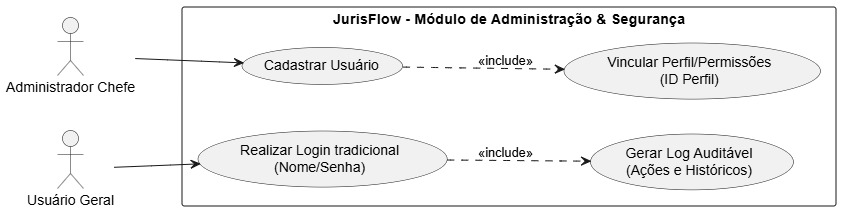
\includegraphics[width=0.9\textwidth]{04-figuras/diagrama1.jpeg}
\end{figure}

A Figura \textcolor{blue}{\ref{fig:1}}apresenta dois atores principais, com responsabilidades distintas
no sistema. O Administrador Chefe é responsável pelo cadastro de novos usuários. Nesse
processo, o caso de uso de cadastro inclui obrigatoriamente a ação de Vincular Perfil
e Permissões, identificada pelo ID do perfil, garantindo que cada usuário cadastrado
tenha as permissões correspondentes ao seu perfil de acesso. O Usuário Geral realiza o
processo de login por meio da inserção de nome e senha. Como mecanismo de segurança
e rastreabilidade, esse processo inclui automaticamente a ação de Gerar Log Auditável,
responsável por registrar as ações realizadas e o histórico de atividades do usuário no
sistema.

\begin{figure}[H]
    \centering
    \caption{Diagrama de casos de uso: Gestão de Clientes, Casos e Processos.}
    \label{fig:2}
    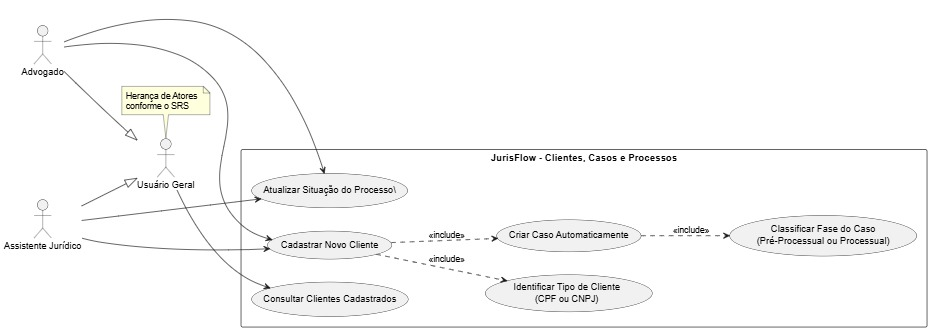
\includegraphics[width=0.9\textwidth]{04-figuras/diagrama2.jpeg}
\end{figure}
Um detalhe importante na modelagem é que tanto o Advogado quanto o Assistente
Jurídico possuem o mesmo nível de acesso e as mesmas permissões dentro deste escopo.
Ambos os profissionais podem Atualizar a Situação do Processo, Consultar Clientes
Cadastrados e iniciar o fluxo de Cadastrar Novo Cliente. Quando um dos profissionais
realiza o cadastro de um novo cliente, o sistema executa obrigatoriamente duas ações:
Identificar o Tipo de Cliente, verificando se o cadastro corresponde a CPF ou CNPJ, e
Criar Caso Automaticamente. Após a criação automática do caso, o sistema também
realiza a etapa de Classificar a Fase do Caso, definindo se o caso se encontra na fase
Pré-Processual ou Processual.

\begin{figure}[H]
    \centering
    \caption{Diagrama de casos de uso: Central de Diligências e Notificações Preventivas.}
    \label{fig:3}
    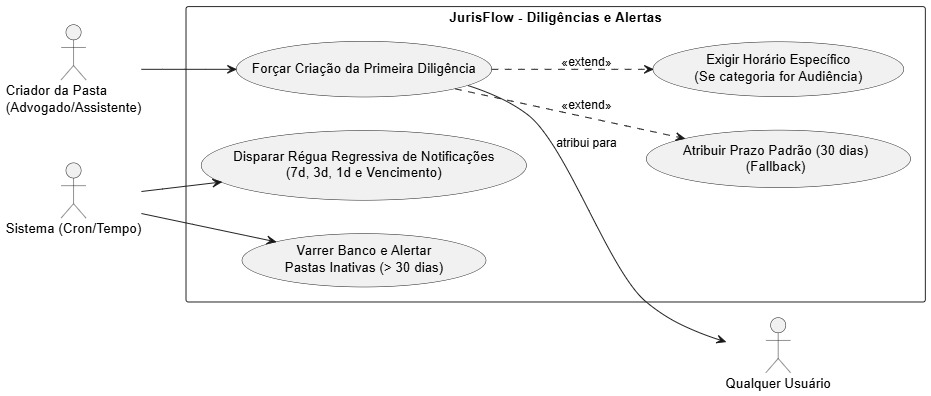
\includegraphics[width=0.9\textwidth]{04-figuras/diagrama3.jpeg}
\end{figure}

O módulo apresenta dois atores responsáveis pela interação direta com suas
funcionalidades, além de um ator de destino relacionado à execução de uma das ações.
Nesse contexto, o Criador da Pasta, representado por um Advogado ou Assistente Jurídico,
é responsável por executar a ação de Forçar Criação da Primeira Diligência, garantindo
que, após a criação da pasta, seja registrada a primeira atividade relacionada ao caso. O
fluxo também contempla duas extensões condicionais baseadas em regras de negócio. A
primeira é Exigir Horário Específico, acionada quando a categoria do caso corresponde a
uma audiência, situação na qual é necessário registrar, além da data, um horário específico
para o compromisso. A segunda é Atribuir Prazo Padrão de 30 dias, utilizada como
comportamento de fallback quando não for informado um prazo maior, garantindo que
nenhuma diligência seja criada sem uma data de vencimento definida. Além dos atores que
interagem diretamente com o módulo, existe o ator Sistema Automatizado, responsável pela
execução de rotinas em segundo plano relacionadas ao controle temporal das atividades.
Entre suas responsabilidades está Disparar a Régua Regressiva de Notificações, enviando
alertas preventivos nos períodos de 7, 3 e 1 dia antes do vencimento, bem como no próprio
dia do vencimento. O Sistema Automatizado também é responsável por Varrer o Banco e
Alertar sobre Pastas Inativas, realizando o monitoramento periódico das pastas e processos
cadastrados. Quando uma pasta permanece sem atualização por período superior a 30
dias, o sistema gera uma notificação para alertar a equipe responsável, contribuindo para
o acompanhamento contínuo dos casos e para a redução de processos sem movimentação.

\begin{figure}[H]
    \centering
    \caption{Diagrama de casos de uso:  Painel Gerencial (Métricas).}
    \label{fig:4}
    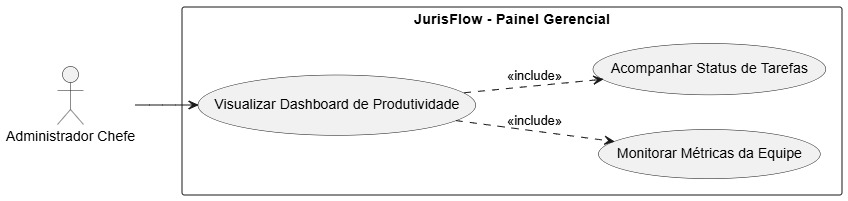
\includegraphics[width=0.9\textwidth]{04-figuras/diagrama4.jpeg}
\end{figure}

Para encerrar a apresentação dos casos de uso, o quarto diagrama representa o
módulo de Painel Gerencial (Métricas) do JurisFlow, destinado ao acompanhamento e à
supervisão das atividades do escritório. Nesse módulo, o Administrador Chefe é o ator
responsável por acessar a funcionalidade Visualizar Dashboard de Produtividade, por
meio da qual são disponibilizadas informações relacionadas ao desempenho da equipe e ao
andamento das atividades.

\section{GESTÃO E ORGANIZAÇÃO DO PROJETO}